\documentclass{beamer}
\author{Ismael Bastos}
\usepackage[portuguese]{babel}
\usepackage{multicol}
\newtheorem{teorema}{Teorema}
\newtheorem{exemplo}{Exemplo}
\newtheorem{definicao}{Definição}
\begin{document}
\section{Introdução à teoria dos conjuntos}
\section{Princípios de Contagem}
\begin{frame}{Princípios de Contagem}
 Os princípios de contagem são a base de toda a aritmética realizada em análise combinatória. Todos os objetos que iremos estudar são construídos a partir de operações de multiplicação e adição que serão definidas a partir dessas duas regras primárias.    
\end{frame}

\begin{frame}{Princípio fundamental da contagem}
    \begin{teorema}
        Considere uma tarefa dividida em dois experimentos. Para o primeiro experimento existem $n_1$ resultados possíveis e para cada resultado do primeiro existem $n_2$ resultados possíveis para o segundo experimento. Dessa forma, o número total de resultados possíveis para a tarefa é:
        $$n=n_1 \cdot n_2$$
    \end{teorema}    
\end{frame}

\begin{frame}{Princípio fundamental da contagem}
\begin{exemplo}
Em um cinema qualquer, a barraca de pipoca exibe as seguintes opções:
    \begin{multicols}{2}
        Tamanho:
        \begin{itemize}
        \item pequena
        \item média
        \item grande
        \item mega
        \end{itemize}
        
        \columnbreak
        
        Cobertura:
        \begin{itemize}
        \item manteiga
        \item chocolate
        \item sem cobertura
        \end{itemize}
    \end{multicols}
    
\text{De quantas maneiras diferentes podemos pedir um balde de pipoca?}
\end{exemplo}
\end{frame}

\begin{frame}{Princípio fundamental da contagem}
\begin{teorema}
    Tomemos agora uma tarefa dividida em $r$ experimentos. Se:
    \begin{itemize}
        \item Para o primeiro experimento há $n_1$ resultados possíveis
        \item Para cada resultado do primeiro há $n_2$ resultados possíveis para o segundo 
        \item Para cada resultado do segundo há $n_3$ resultados possíveis para o terceiro
        \item e assim sucessivamente até o r-ésimo experimento
    \end{itemize}
    Então existem
    $$n = n_1 \cdot n_2 \cdot \dots \cdot n_r$$
\end{teorema}
    
\end{frame}

\begin{frame}
    \begin{exemplo}
        Quantos números de 5 algarismos podemos escrever de forma que o primeiro algarismo seja par, o segundo seja ímpar, o terceiro seja múltiplo de 3 e não hajam restrições para o quarto e o quinto?
    \end{exemplo}
\end{frame}

\begin{frame}{Princípio fundamental da contagem}
\begin{exemplo}
O RNA, ou Ácido Ribonucleico, é uma molécula constituída de uma longa "fita" a qual se conecta uma longa sequência de bases nitrogenadas. Essas bases podem ser uma das seguintes quatro moléculas:
\begin{itemize}
    \item Adenina (A)
    \item Uracila (U)
    \item Citosina (C)
    \item Guanina (G)
\end{itemize}
Um códon é uma trinca (sequência de três) dessas quatro bases e cada códon está ligado a um comando na cadeia produtora de aminoácidos (mais de um códon pode corresponder corresponder ao mesmo aminoácido). Quantos códons diferentes podem ser formados a partir do RNA?
\end{exemplo}
\end{frame}

\begin{frame}{Princípio aditivo}

\begin{teorema}
    Se uma tarefa consiste em realizar um experimento experimento $E_1$ com $n_1$ resultados possíveis ou um segundo experimento $E_2$ com $n_2$ resultados possíveis e os conjuntos de resultados $E_1$ e $E_2$ são disjuntos, então o número total de resultados dessa tarefa é:
    $$n = n_1 + n_2$$
\end{teorema}
    \begin{exemplo}
        Suponha que uma sorveteria venda sorvetes e açaí. O cliente pode comprar um sorvete no pote ou na casquinha, podendo escolher um sorvete pequeno, médio ou grande entre 28 sabores e três cobertura. Se o cliente preferir um açaí ele tem 4 tamanhos diferentes e pode escolher 7 opções de recheio. Quantas escolhas o cliente tem se ele quer:
        \begin{enumerate}
            \item Um sorvete E um açaí
            \item Um sorvete OU um açaí
        \end{enumerate}
    \end{exemplo}
\end{frame}

\begin{frame}{Princípio aditivo}

Assim como fizemos para o princípio multiplicativo, podemos também generalizar o conceito aditivo para mais de dois experimentos.

\begin{teorema}
    Tomemos uma tarefa dividida em r experimentos, $E_1, E_2, \dots, E_r$ com as seguintes regras:
    \begin{itemize}
        \item $A_i$ é o conjunto de resultados possíveis de $E_i$ para $i=1, \dots, r$
        \item$ A_1, A_2, \dots, A_r$ são disjuntos dois a dois
    \end{itemize}

    Então o número total de resultados da tarefa é:
    $$\left| \cup_{i=1}^r A_i\right| = \sum_{i=1}^{r} |A_i| = |A_i| + |A_2| + \dots + |A_r|$$
    
\end{teorema}

    
\end{frame}

\begin{frame}{Princípio aditivo}

\begin{exemplo}
    Uma companhia de viagens resolveu dividir seus destinos em 3 categorias:
    \begin{itemize}
        \item Categoria 1: Praias (40 destinos)
        \item Categoria 2: Grandes Cidades (15 destinos)
        \item Categoria 3: Cidades Históricas (32 destinos)
    \end{itemize}

    A companhia também resolveu vender pacotes de viagem no seguinte formato: Você escolhe duas categorias dessas três e então um destino em cada categoria. Supondo que o mesmo destino não pode aparecer em mais de uma categoria, quantos pacotes diferentes podem ser formados nesse formato? 
    
\end{exemplo}
\end{frame}

\begin{frame}{Permutações}
    Dada uma sequência $x=x_1x_2x_3 \dots x_r$ uma permutação de $x$ é qualquer reordenação dessa sequência 

    \begin{exemplo}
    \begin{itemize}
        \item (5,6,3,1,2,4) é uma permutação de (1,2,3,4,5,6). Vale também dizer que o contrário vale.
        \item (R,I,V,A,L) é uma permutação de (V,I,R,A,L)
        \item (2,3,0,2) e (3,2,0,2) são permutações de (2,0,2,3)
        \item O conjunto de permutações formadas a partir do conjunto $\{1,2,3,4\}$ contém as seguintes sequências:
        \begin{figure}
            \centering
            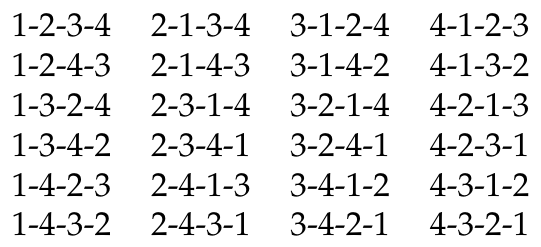
\includegraphics[width=0.5\linewidth]{figures/pem_1234.png}
        \end{figure}
    \end{itemize}
    \end{exemplo}
\end{frame}

\begin{frame}{Permutações}
    Na maior parte do tempo não estamos interessados no conjunto das permutações, mas sim no número de permutações possíveis a partir de um conjunto ou de uma sequência.

    \begin{teorema}
        O número de permutações de uma sequência ou de um conjunto com $n$ elementos distintos é dado por:
        $$PM_n := n \cdot (n-1) \cdot (n-2) \cdot \dots \cdot 2 \cdot 1$$
    \end{teorema}

    \textbf{Notação:} Usamos a seguinte notação para facilitar a escrita do produtório:
    $$n! = n \cdot (n-1) \cdot (n-2) \cdot \dots \cdot 2 \cdot 1$$
Chamamos $n!$ de "$n$ fatorial" ou de "fatorial de $n$"
\end{frame}

\begin{frame}{Permutações}

\begin{exemplo}
    Em uma escola de música, quatro professores multi-instrumentistas resolveram preparar uma apresentação na qual cada música contaria com os quatro tocando em uma formação diferente os seguinte instrumentos: Teclado, Guitarra, Baixo e Bateria. Qual o número máximo de músicas a serem tocadas?
\end{exemplo}
    \pause
    \begin{exemplo}
        De quantas formas diferentes podemos rearranjar 6 vagões de um trem?
    \end{exemplo}
\end{frame}

\begin{frame}{Permutações}
\textbf{Propriedades dos fatoriais}

Dados $n$ inteiro positivo, então as seguintes propriedades são validas:

\begin{enumerate}
    \item $n! = n \cdot (n-1)!$
    \item $(n-1)! = \dfrac{n!}{n}$
    \item $0! = 1$
\end{enumerate}
\end{frame}
 \begin{frame}{Permutações}
 \textbf{Anagramas}

 Um caso especial de permutação é a reordenação das letras em uma palabra, ou anagrama:

 \begin{exemplo}
     \begin{itemize}
         \item AMOR e OMAR são anagramas da palavra ROMA
         \item ARTE, TERA, TEAR e RETA são anagramas entre si
         \item CASA, ASAC, SACA são anagramas entre si
     \end{itemize}
 \end{exemplo}
     \textcolor{red}{Importante} Assim como pode ser observado no terceiro exemplo, os anagramas não precisam ser palavras do vocabulário real.
 \end{frame}   

\begin{frame}{Permutações}
\begin{teorema}
    O número de anagramas para uma palavra com $n$ letras diferentes é dado por:
    $$AN_n = n!$$
\end{teorema}

\begin{exemplo}
    \begin{itemize}
        \item A palavra CÉU tem $3!$ anagramas.
        \item A palavra PEDAL tem $5!$ anagramas.
        \item A palavra JÚPITER tem $7!$ anagramas.
        \item A palavra PERNAMBUCO tem $10!$ anagramas
    \end{itemize}
    \textcolor{red}{Importante}: O que acontece se tivermos letras repetidas na palavra?
\end{exemplo}
\end{frame}

\begin{frame}{Permutações}
    Para responder essa pergunta, tomemos como exemplo a palavra ANO, claramente nessa palavra não existe repetição de letra, logo, sabemos que existem $3!$ anagramas, sendo eles.

    $$ANO, AON, NAO, NOA, OAN, ONA $$
\pause    
    Agora tomemos a palavra ANA, note que os possíveis anagramas são os mesmos que da palavra ANO, mas trocando a letra O pela letra A. 

   $$ ANA, AAN, NAA, NAA, AAN, ANA$$
\pause
    Perceba que agora temos todos os anagramas aparecendo duas vezes, entretanto, dois anagramas iguais são o mesmo anagrama. Logo, o número de anagramas da palavra ANA é 3.
\end{frame}

\begin{frame}{Permutações}

Perceba que o mesmo ocorre para as palavras BOLA e BALA. BOLA tem $4!$ possíveis permutações, sendo elas

$$BOLA, BOAL, BALO, BAOL, BLOA, BLAO$$
$$OBLA, OBAL, OLBA, OLAB, OALB, OABL$$
$$ALOB, ABOL, ABLO, AOLB, ALBO, AOBL$$
$$LBOA, LBAO, LOAB, LOBA, LABO, LAOB $$

\pause
Para obtermos os anagramas da palavra BALA, basta trocar onde aparece letra O pela letra A. 

$$BALA, BAAL, BALA, BAAL, BLAA, BLAA$$
$$ABLA, ABAL, ALBA, ALAB, AALB, AABL$$
$$ALAB, ABAL, ABLA, AALB, ALBA, AABL$$
$$LBAA, LBAA, LAAB, LABA, LABA, LAAB $$
\end{frame}

\begin{frame}{Permutações}
\begin{teorema}
    Se uma palavra de $r$ letras é composta pelas letras $a_1, \dots, a_r$ em que a letra $a_i$ aparece $n_i$ vezes para todo $i$ entre 1 e $r$, então o número de anagramas dessa palavra é:

    $$AN_{n_1, n_2, \dots, n_r} = \dfrac{n!}{n_1! \cdot n_2! \cdot \dots \cdot n_r!}$$
\end{teorema}

   \begin{exemplo}
   \begin{itemize}
       \item Calcule o número de anagramas da palavra PAPA.
       \item Calcule o número de anagramas da palavra MATEMÁTICA.
       \item Calcule o número de anagramas da palavra ESTATÍSTICA.
   \end{itemize}   
   \end{exemplo}
\end{frame}

\begin{frame}{Permutações}

\textbf{Permutações Dentro e Entre}
    Algumas vezes os objetos a serem permutados podem se dividir em duas ou mais categorias eo problema em questão nos pede para levar em conta as categorias na contagem.
    \begin{exemplo}
        Um estudante de filosofia possui 10 livros diferentes
        \begin{itemize}
            \item 4 de ética
            \item 3 de epistemologia
            \item 2 de lógica
            \item 1 de fenomenologia
        \end{itemize}

        De quantas formas diferentes ele pode ordenar seus livros em sua estante se:
        \begin{enumerate}
            \item Ele não tem nenhuma restrição.
            \item Os livros da mesma área são indistinguíveis entre si.
            \item Os livros de ética devem ser colocados primeiro, então os de epistemologia, os de lógica e por fim o de fenomenologia.
        \end{enumerate}
    \end{exemplo}
\end{frame}

\begin{frame}{Permutações}
    \begin{exemplo}
        Oito estudantes devem se sentar em 8 cadeiras para a realização de uma prova. 4 desses estudantes são do curso de matemática e 4 são do curso de administração. De quantas formas podemos enfileirar esses estudantes se:
        \begin{enumerate}
            \item Não temos nenhuma restrição
            \item Os estudantes devem ser intercalados por curso.
        \end{enumerate}
    \end{exemplo}
\end{frame}

\begin{frame}{Combinações}
    Em combinatória, nem sempre estamos interessados em ordenar elementos. Podemos também estar interessados em formar combinações, ou seja, subconjuntos (grupos) de tamanho definido partindo de um conjunto inicial. 
    \pause
    \begin{teorema}
        Tome $S$ um conjunto de tamanho $n$ qualquer, o número de combinações de tamanho $k$ a  partir de $S$ é dado por:
        $$C_{n,k} = \binom{n}{k} = \dfrac{n!}{k!(n-k)!}$$
    \end{teorema}

    \pause
    \begin{exemplo}
        De um grupo de 10 crianças precisamos selecionar 3 para um projeto de leitura. De quantas formas podemos fazer essa seleção?
    \end{exemplo}
\end{frame}

\begin{frame}{Combinações}

\begin{exemplo}
    Se uma companhia aérea tem 40 destinos e quer vender pacotes que passam por 5 deles, qual o número de pacotes possíveis que essa empresa pode montar?
\end{exemplo}

\pause
\begin{exemplo}
    Se uma caixa tem 15 lampadas (10 em perfeitas condições e 5 queimadas) e selecionamos 6 delas. Qual o número de combinações em que 4 dessas lampadas estão queimadas?
\end{exemplo}
\pause
\begin{exemplo}
    Dada a mesma caixa do exemplo anterior. Qual o número de combinações possíveis em que 1 ou 2 lampadas estão queimadas?
\end{exemplo}
\end{frame}

\begin{frame}{Arranjos}
Sabendo reordenar todos os elementos de uma sequência e destacar subconjuntos a partir de um conjunto maior, podemos combinar essas duas ações e reordenar apenas alguns elementos de um conjunto

\begin{teorema}
    Dado um conjunto S com $|S|=n$, o número de arranjos de tamanho $r \leq n$ a partir de S é:
    $$AR_{n,r} = \dfrac{n!}{(n-r)!}$$
\end{teorema}
\end{frame}

\begin{frame}{Arranjos}
    \begin{exemplo}
        Quantas placas de carro podemos formar no antigo modelo brasileiro (3 letras e 4 números) se:

        \begin{enumerate}
            \item Não temos restrições. 
            \item As letras não podem se repetir
            \item Os números não podem se repetir
            \item Nem letras nem números podem se repetir
        \end{enumerate}
    \end{exemplo}
\end{frame}

\begin{frame}{Arranjos}
\begin{exemplo}
    De um grupo de 40 alunos, espera-se formar um comitê de 6 pessoas. De quantas formas é possível formá-lo se:
    \begin{enumerate}
        \item Não há regras especiais na seleção
        \item Temos que escolher um líder no comitê
        \item Temos que escolher um líder, um vice-líder e um tesoureiro dentro do comitê.
    \end{enumerate}
\end{exemplo}
\end{frame}

\begin{frame}{Arranjo X Combinação}

Devemos usar arranjo quando desejamos formar grupos em que a ordem importa e combinações quando a ela não importa, mas essa resposta só apresenta metade do caminho. 

\vspace{3px}
\pause

Usamos combinações quando o problema nos pede para escolher, selecionar, formar grupos, formar subconjuntos ou formar objetos que são coleções de elementos (como times, pacotes, comitês, etc...) sem dar aos elementos uma característica ou posição depois da seleção.

\vspace{3px}
\pause

Usamos arranjos quando o problema nos pede para enfileirar, ordenar, formar sequências, formar ordend, formar filas, formar objetos que são sequências de elementos (como palavras, placas de carro, números etc...) 0ou dar uma característica especial ou posição para cada elemento do subconjunto que retiramos do conjunto inicial. 
    
\end{frame}

\begin{frame}{Soluções inteiras de equações}

Estamos interessados em saber quantas soluções uma equação da forma

$$x_1 + x_2 + \dots + x_n = n$$

possui, onde as variáveis $x_1, x_2, \cdot, x_r$ tomam valores inteiros positivos $(1,2,3,\dots)$ ou inteiros não-negativos $(0,1,2,3,\dots)$
\end{frame}

\begin{frame}{Soluções inteiras positivas}

\begin{definicao}
    O número de soluções inteiras positivas para a equação:
    $$x_1 + x_2 + \dots + x_r = n$$
    é dado por:

    $$\binom{n-1}{r-1}$$
\end{definicao}
\end{frame}

\begin{frame}{Soluções inteiras positivas}

\begin{exemplo}
    Um investidor possui dez mil reais e deseja investir em três empresas. Quantas carteiras de investimento ele pode criar sele só pode investir em incrementos de mil reais e ele deve investir pelo menos mil reais em cada uma?
\end{exemplo}

\pause

\begin{exemplo}
    Quantas soluções diferentes tem a equação:
    $$x_1 + x_2 = 5$$
\end{exemplo}
\end{frame}

\begin{frame}{Soluções inteiras não-negativas}
    \begin{teorema}
        O número de soluções inteiras não-negativas para uma equação da forma:

        $$x_1+x_2+\dots+x_r = n$$
        é dado por:
        $$\binom{n+r-1}{r-1}$$
    \end{teorema}
\end{frame}

\end{document}
